\documentclass[a4paper,11pt]{article}

% Identificação
\newcommand{\pbtitulo}{Modelo C4}
\newcommand{\pbversao}{1.0}

\usepackage{../sty/tutorial}
\usepackage{tabularx}
\usepackage{longtable}
\usepackage{booktabs}
\usepackage{caption}

%----------------------------------------------------------------------
% Início do Documento
%----------------------------------------------------------------------
\begin{document}
	
\maketitle % mostrar o título
\thispagestyle{fancy} % habilitar o cabeçalho/rodapé das páginas

%----------------------------------------------------------------------
% RESUMO DO ARTIGO
%----------------------------------------------------------------------

\begin{abstract}	
	\initial{A}rquitetos de software são os profissionais que planejam e organizam sistemas complexos -- como aplicativos, sites e redes. Administram desde a estrutura, segurança e o funcionamento dessas soluções. Assim como um arquiteto de obras usa plantas e documentos
	técnicos para orientar a construção de um prédio, o arquiteto de software necessita de diagramas e representações visuais para facilitar o entendimento de sistemas tecnológicos. \textbf{Modelo C4} é uma forma simples e poderosa de comunicar a arquitetura de um sistema de software em diferentes níveis de detalhe. Permite que contemos variadas histórias para públicos diferentes -- desde uma visão geral para gestores e analistas, até os detalhes técnicos para desenvolvedores.
\end{abstract}

%----------------------------------------------------------------------
% CONTEÚDO DO ARTIGO
%----------------------------------------------------------------------
\section{Introdução}
Por muitos tempo, arquitetura significou projetar e construir estruturas físicas, como casas e edifícios. Mas, nas últimas d´ecadas, os termos arquitetura e arquiteto passaram a serem utilizados também no mundo da tecnologia e do desenvolvimento de software. O grande problema é que, diferente da engenharia civil, os profissionais de software nem sempre seguem um padrão visual. Cada empresa ou mesmo analista utiliza de símbolos, formas e cores diferentes, o que pode gerar confusão, principalmente para quem não é da área técnica

Diagramas de arquitetura de software são uma excelente forma de mostrar como um sistema será
construído (durante o planejamento) ou como funciona atualmente (para documentar, compartilhar
conhecimento ou treinar pessoas). Porém, é bem provável que muitos dos diagramas de software que já tenhamos visto se pareçam apenas um emaranhado confuso de caixas e setas, sem muito sentido. Isso acontece porque, com a popularização das metodologias ágeis — como prega o Manifesto Ágil – muitas equipes deixaram de lado (ou reduziram bastante) o hábito de documentar seus sistemas de forma organizada, inclusive com diagramas \textbf{UML}, que antes eram comuns. 

O que vemos hoje, são equipes que costumam improvisar diagramas de última hora, feitos às pressas em quadros brancos ou em ferramentas genéricas como o DrawIO\cite{drawio}. O maior problema é a falta de padrões claros, cada um faz do seu jeito\footnote{Gera confusão e dificulta o entendimento, principalmente para quem não participou da criação do sistema}.

No ano passado, o especialista \textbf{Ionut Balosin} escreveu o artigo ”A Arte de Criar Diagramas Arquiteturais\footnote{Disponível em: \url{https://www.infoq.com/articles/crafting-architectural-diagrams/}}", onde destaca vários problemas comuns nesse tipo de prática, como o uso de símbolos confusos e a falta de clareza no que cada elemento do diagrama representa.

\section{Modelo C4}
Este modelo foi criado por \textbf{Simon Brown} desenvolvido justamente para acabar com essa bagunça e tornar a comunicação da arquitetura de software mais clara e acessível -- mesmo para quem não é especialista no assunto.

\begin{figure}[!htb]
	\centering
	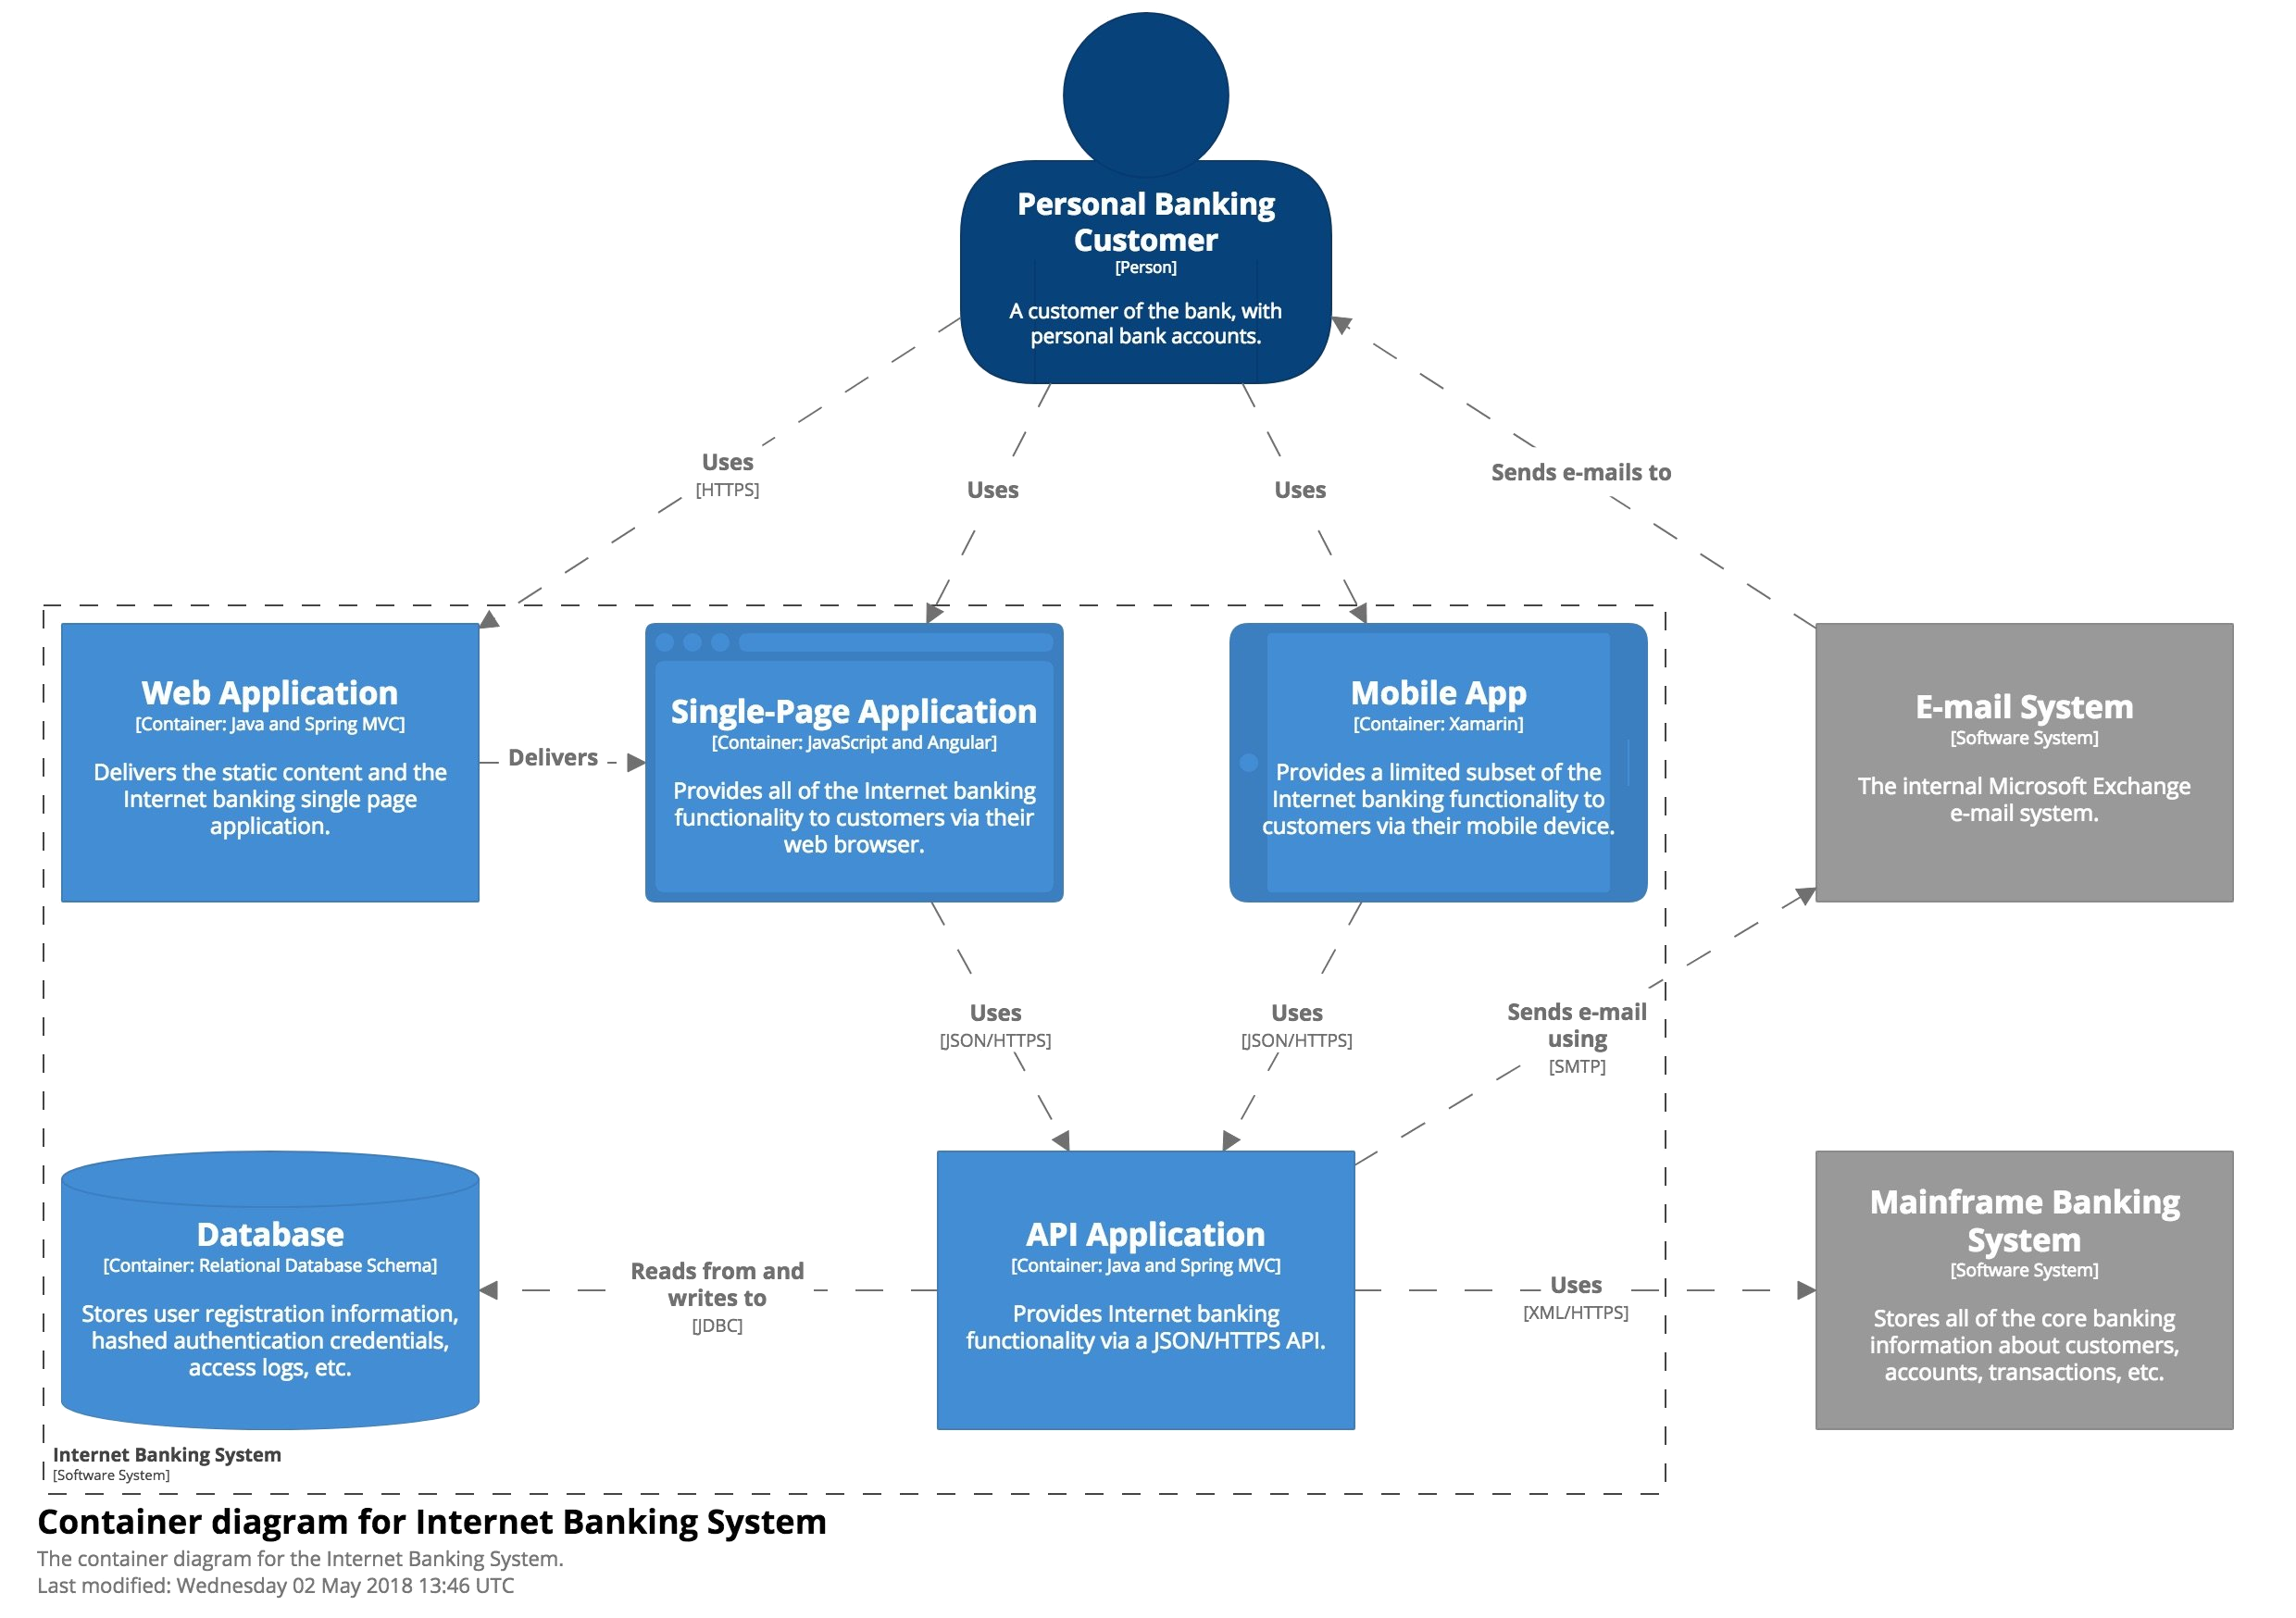
\includegraphics[width=0.9\textwidth]{imagens/ModeloC4}
	\caption{Exemplo do Modelo C4}
\end{figure}

O nome \textbf{Modelo C4} vem das palavras: Contexto, Contêineres, Componentes e Código -- quatro níveis de diagramas que auxiliam a visualizar um sistema de forma progressiva, como se estivesse aproximando ou afastando o zoom no \textit{Google Maps}. Cada nível tem seu propósito e é mais adequado para públicos diferentes – desde gestores e analistas até desenvolvedores.

Mas, para criar esse “mapa do seu sistema”, primeiro é preciso falar uma mesma linguagem. Significa usar conceitos padronizados, que todos compreendam. \textbf{Modelo C4} ajuda justamente por oferecer uma maneira consistente ao descrever uma estrutura estática de um sistema, ou seja, o que o compõe, como está organizado e como funciona por trás dos bastidores.
O modelo considera os seguintes elementos:
\begin{itemize}
	\item \textbf{Contêineres}: grandes blocos do sistema, como aplicativos, bancos de dados e microserviços;
	\item \textbf{Componentes}: partes internas de cada contêiner, que executam funcionalidades específicas;
	\item \textbf{Código}: nível mais detalhado, voltado aos desenvolvedores;
	\item \textbf{Pessoas}: usuários que interagem com tudo isso.
\end{itemize}

\section{Visão Geral do Modelo C4}
Como já descrito na seção anterior, o Modelo C4 possui quatro níveis, do mais amplo ao mais
detalhado:

\begin{table}[H]
	\centering 
	\begin{tabular}{C{2.3cm} | C{5.5cm} | C{5cm} }
		\textbf{Nível} & \textbf{O que mostra?} & \textbf{Para quem é indicado?} \\
		Contexto & Como o sistema se encaixa no mundo -- quem o usa, como se conecta com outros sistemas. & Para gestores, analistas, usuários, e novos integrantes da equipe. \\
		Contêineres & Quais são os principais blocos que compõem o sistema (apps, serviços,
		banco de dados) e como eles se comunicam. & Para arquitetos, líderes técnicos e desenvolvedores. \\
		Componentes & Como cada contêiner é dividido internamente: módulos, APIs, classes principais. & Para desenvolvedores e equipe técnica.  \\
		Código & O nível mais detalhado: classes, arquivos, métodos. & Para desenvolvedores
		experientes. \\
	\end{tabular}
\end{table}

\textbf{Modelo C4} é formado por um conjunto de diagramas que mostram diferentes níveis de detalhe sobre o seu sistema. Cada diagrama apresenta uma visão específica, facilita a compreensão das ideias de forma visual e acessível. Com isso, qualquer pessoa pode "dar um zoom" nas partes que mais interessam e entender tanto a visão geral quanto os detalhes do funcionamento do software.

Vamos entender com a seguinte analogia: \textbf{Modelo C4} é como um mapa de uma cidade, mas
voltado para sistemas de software. Utiliza-se de um conjunto de diagramas que mostram o sistema
em diferentes níveis de detalhe -- desde a visão mais ampla até os componentes internos.

Imaginemos olhar um mapa: começamos com o país (visão geral), depois a cidade (estrutura
principal), em seguida os bairros (módulos do sistema) e, por fim, as ruas e casas (os detalhes do código). O modelo permite que qualquer pessoa -- mesmo sem conhecimento técnico profundo -- consiga entender o funcionamento do sistema, explorar as partes que mais interessam com clareza e facilidade.

Sempre incluamos legenda nos seus diagramas -- mesmo que a simbologia pareça óbvia. Essa legenda deve explicar os significados das cores, formas, siglas, estilos de linha, bordas, tamanhos e qualquer outro elemento visual utilizado. 

Fazendo assim, auxiliamos quem está vendo o diagrama a entender rapidamente como interpretar a imagem, sem precisar adivinhar. É importante manter esse padrão consistente em todos os níveis do \textbf{Modelo C4}, para que a leitura seja clara e intuitiva do início ao fim.

\subsection{Nível 1 - Diagrama de Contexto}
Mostra o sistema como um todo, quem o usa e com o que interage. Por exemplo: Imaginemos um
sistema chamado ”Gestor de Biblioteca Online”. \vspace{-1em}
\begin{verbatim}
[Usuário] <--> [Sistema de Biblioteca]
[Sistema de Biblioteca] <--> [Sistema de Pagamento]
[Sistema de Biblioteca] <--> [Serviço de E-mail]
\end{verbatim}

\begin{figure}[!htb]
	\centering
	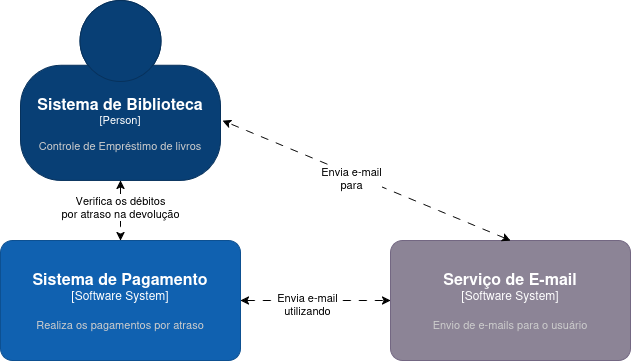
\includegraphics[width=0.6\textwidth]{imagens/Contexto}
	\caption{Diagrama de Contexto}
\end{figure}

Aqui mostramos que o usuário interage com o sistema de biblioteca, que por sua vez se conecta com outros sistemas, como pagamento e envio de e-mails. Nenhum detalhe técnico ainda — apenas o
panorama geral. Esse nível do modelo C4 oferece-nos uma visão panorâmica do sistema – como se fosse uma foto tirada de cima, mostrar tudo de forma ampla. O objetivo aqui, não é entrar nos detalhes técnicos ou na forma como tudo funciona por dentro, mas apresentar o sistema de maneira geral: o que faz, quem o utiliza e com quais outros sistemas no qual se conecta.

Esse tipo de diagrama é ideal para compartilhar com públicos não técnicos, como gestores ou
analistas de negócio. Auxilia-nos a entender o escopo do projeto, quem são os usuários e qual
problema o sistema busca resolver. Em resumo, mostra como esse sistema se encaixa dentro do
ambiente de TI da organização – como a peça de um quebra-cabeça maior.

\subsection{Nível 2 - Diagrama de Contêineres}
Abrimos o sistema para ver os principais blocos que o compõem. Por exemplo: Como funciona a
comunicação do "Aplicativo Web". \vspace{-1em}
\begin{verbatim}
[Aplicativo Web] <--> [API REST] <--> [Banco de Dados]
                            |
                            +--> [Serviço de E-mail]
\end{verbatim}

\begin{figure}[!htb]
	\centering
	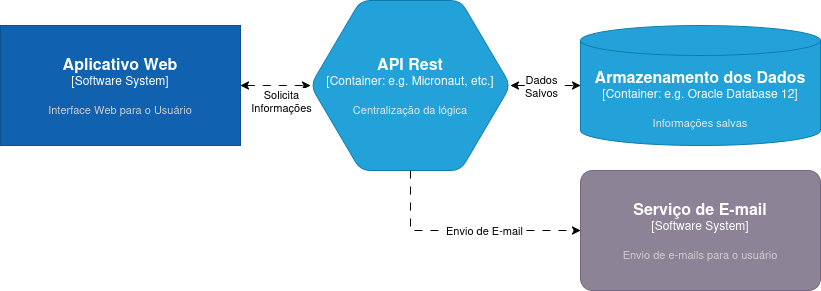
\includegraphics[width=0.8\textwidth]{imagens/Conteiners}
	\caption{Diagrama de Contêineres}
\end{figure}

Estamos observando que há uma interface Web, uma API que centraliza a lógica, um banco de
dados onde as informações ficam guardadas, e um serviço auxiliar para envio de e-mails. Esse diagrama representa o próximo nível de detalhe do sistema. Mostra os "contêineres", ou seja, as partes principais que compõem o sistema, como funcionam e se comunicam entre si.

Podemos imaginar os contêineres como "caixas organizadas", cada uma com tudo o que precisa
para funcionar: códigos, bibliotecas, arquivos de configuração e dados. Um contêiner pode ser, por exemplo, um aplicativo de celular, um site que roda no servidor ou um programa instalado em um computador.

Essas caixas são preparadas para serem executadas em diferentes ambientes (como servidores, nuvens ou dispositivos), e o diagrama ajuda a visualizar como essas partes se conectam para formar o sistema completo.

\subsection{Nível 3 - Diagrama de Componentes}
Neste nível, mergulhamos dentro de um contêiner (ex: a API) para entender suas partes internas.
Por exemplo: Por dentro da API REST \vspace{-1em}
\begin{verbatim}
[Controle de Usuários] <--> [Serviço de Autenticação]
                              |
                              +--> [Gerenciador de Livros]
                              +--> [Gestor de Reservas]
\end{verbatim}

\begin{figure}[!htb]
	\centering
	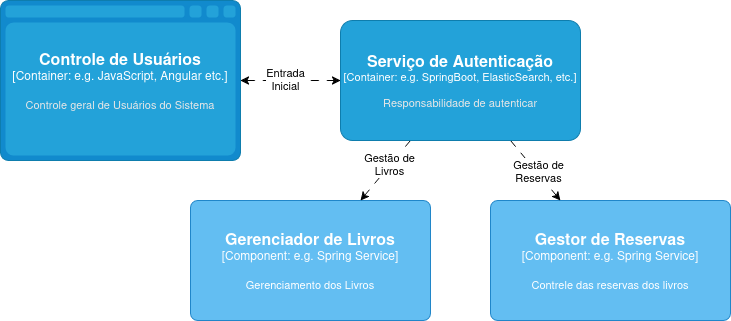
\includegraphics[width=0.8\textwidth]{imagens/Componentes}
	\caption{Diagrama de Componentes}
\end{figure}

Cada "componente" torna-se uma parte com uma função clara: autenticar, cadastrar livros, controlar reservas. \textbf{Diagrama de componentes} aprofunda ainda mais a visão do sistema, mostrar o que existe dentro de cada contêiner (aquelas ”caixas” do nível anterior). Divide o conteúdo de cada contêiner em partes menores – como blocos de construção – que representam os arquivos, bibliotecas, pedaços de código e funções que fazem aquele contêiner funcionar.

Esse tipo de diagrama mostra com clareza o papel de cada componente, como se conectam e quais
tecnologias estão envolvidas. Imaginemos isso como abrir um aparelho eletrônico: o contêiner seria esse aparelho em si, e o diagrama de componentes revela as peças internas, analisar como cada uma contribui para o funcionamento do todo.

Esses diagramas ajudam muito a equipe técnica a entender melhor a estrutura do sistema, facilita o desenvolvimento, manutenção e evolução do software. Com esse modelo, fica muito mais fácil explicar como o sistema funciona, seja para quem entende de tecnologia ou para quem precisa apenas enxergar o panorama geral do projeto.

\subsection{Nível 4 - Diagrama de Código}
Este é o nível mais técnico: mostra o código em si. Por exemplo, as classes que formam o componente "Gerenciador de Livros".
 \vspace{-1em}
\begin{verbatim}
+ LivroController
+ LivroService
+ LivroRepository
+ Livro (classe modelo)
\end{verbatim}

\begin{figure}[!htb]
\centering
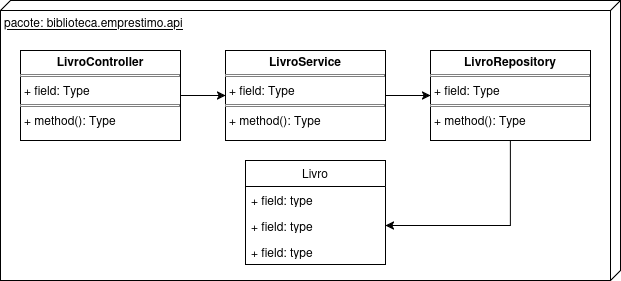
\includegraphics[width=0.8\textwidth]{imagens/Codigo}
\caption{Diagrama de Codigo}
\end{figure}

Esse nível ajuda desenvolvedores a entender como o código está organizado e como cada classe se
conecta. Nesse último nível, o zoom vai até o código-fonte de cada componente. É aqui que vemos como cada parte do sistema foi escrita e implementada em linguagem de programação.

Esse nível é representado pelo \textbf{Diagrama de Classes UML}\footnote{Meio visual de mostrar como o código está estruturado}. Uma classe funciona como uma planta de construção: define como certos ”objetos” devem ser montados, quais características (atributos) possuem e o que são capazes de fazer (operações ou comportamentos).

É como olhar o projeto técnico de uma máquina: vemos o detalhe de cada peça e como deve funcionar. Para desenvolvedores, esse nível é essencial para garantir que tudo esteja bem organizado e corretamente funcional.

\section{Conclusão}
Assim temos os seguintes benefícios na adoção do \textbf{Modelo C4}:
\begin{itemize}
	\item Clareza: Cada nível fala com um público específico.
	\item Padronização: Usa sempre os mesmos conceitos.
	\item Acessibilidade: Até quem não é técnico entende os níveis superiores.
	\item Escalabilidade: Funciona tanto em sistemas pequenos quanto gigantes.
\end{itemize}

\textbf{Modelo C4} não exige o uso de uma notação específica. Os exemplos geralmente usam uma forma simples de representação, que funciona muito bem em quadros brancos, papel, post-its, cartões ou ferramentas digitais de diagramação. Mas, se preferir, podemos usar notações mais formais, como a UML, com seus pacotes, componentes e símbolos padronizados\footnote{Todos modelos gerados nesta apostilas foram realizados utilizou-se do software DrawIO\cite{drawio}}.

Independentemente do estilo escolhido, é recomendável que cada elemento do diagrama tenha
algumas informações essenciais: um nome claro, o tipo de elemento (como “Pessoa”, “Sistema de
Software”, “Contêiner” ou “Componente”), a tecnologia utilizada (se for relevante) e uma breve
descrição\footnote{Podemos consultar mais detalhes na documentação oficial do modelo\cite{c4}}.

Pode até parecer estranho colocar tanto texto em um diagrama, mas isso ajuda a evitar mal-entendidos. Afinal, um bom diagrama de arquitetura não deve deixar espaço para dúvidas -- necessita comunicar de forma clara para todos os envolvidos, técnicos ou não.

Sou um entusiasta do mundo \textbf{Open Source} e novas tecnologias. Qual a diferença entre Livre e Open Source? \underline{Livre} significa que esta apostila é gratuita e pode ser compartilhada a vontade. \underline{Open Source} além de livre todos os arquivos que permitem a geração desta (chamados de arquivos fontes) devem ser disponibilizados para que qualquer pessoa possa modificar ao seu prazer, gerar novas, complementar ou fazer o que quiser. Os fontes da apostila (que foi produzida com o LaTex) está disponibilizado no GitHub \cite{github}. Veja ainda outros artigos que publico sobre tecnologia através do meu Blog Oficial \cite{fernandoanselmo}.

%-----------------------------------------------------------------------------
% REFERÊNCIAS
%-----------------------------------------------------------------------------
\begin{thebibliography}{7}
  \bibitem{c4} 
  Site oficial do C4 Model \\
  \url{https://c4model.com/}

  \bibitem{drawio} 
  Site oficial do DrawIO \\
  \url{https://www.drawio.com/}
  
  	\bibitem{fernandoanselmo} 
	Fernando Anselmo - Blog Oficial de Tecnologia \\
	\url{http://www.fernandoanselmo.blogspot.com.br/}
	
	\bibitem{publicacao} 
	Encontre essa e outras publicações em \\
	\url{https://cetrex.academia.edu/FernandoAnselmo}
	
	\bibitem{github} 
	Repositório para os fontes da apostila \\
	\url{https://github.com/fernandoans/publicacoes}
\end{thebibliography}

\end{document}
